\begin{figure}
    \centering
    \begin{subfigure}{.29\linewidth}
        \centering
        \vspace{-0.5\baselineskip}
        \hspace{-1.5em}
        \begin{tikzpicture}[hypergraph,xscale=1,yscale=0.8,trim left=0cm,trim right=0cm]
            \node[vertex,label={west:$x_1$}] (x1) at (-1, 0) {};
            \node[vertex,label={west:$x_2$}] (x2) at (0, 0) {};
            \node[vertex,label={west:$x_3$}] (x3) at (1, 0) {};
            \node[vertex,label={west:$x_4$}] (x4) at (-1, -1) {};
            \node[vertex,label={west:$x_5$}] (x5) at (-1, -2) {};
            \node[vertex,label={east:$x_6$}] (x6) at (0, -2) {};
            \node[vertex,label={west:$x_7$}] (x7) at (2, 0) {};
        
            \begin{scope}[on background layer]
                    
                \newcommand*{\pathri}{	($(x1) + (-0.2,0.4)$)
    					to[out=0,in=180] ($(x3) + (-0.1,0.4)$)
    					to[out=0,in=90] ($(x3) + (0.3,0)$)
    					to[out=-90,in=0] ($(x3) + (-0.1,-0.4)$)
    					to[out=180,in=0] ($(x1) + (-0.2,-0.4)$)
    					to[out=180,in=-90] ($(x1) + (-0.6,0)$)
    					to[out=90,in=180] ($(x1) + (-0.2,0.4)$)}

                \newcommand*{\pathrii}{	($(x1) + (0.25,0.25)$)
                    to[out=135,in=135] ($(x5) + (-0.25,-0.25)$)
                    to[out=-45,in=-45] ($(x1) + (0.25,0.25)$)}
                
                \newcommand*{\pathriii}{($(x5) + (-0.6,0)$)
        					to[out=90,in=90] ($(x6) + (0.6,0)$)
        					to[out=-90,in=-90] ($(x5) + (-0.6,0)$)}
                
                \newcommand*{\pathriv}{($(x3) + (-0.25,0)$)
                    to[out=90,in=90] ($(x7) + (0.25,0)$)
                    to[out=-90,in=-90] ($(x3) + (-0.25,0)$)}
                
                \draw[hyperedge,looseness=1,draw=Red,fill=Red,fill opacity=.1] \pathri;
                \draw[hyperedge,looseness=1,draw=Fuchsia,fill=Fuchsia,fill opacity=.1] \pathrii;
                \draw[hyperedge,looseness=1,draw=NavyBlue,fill=NavyBlue,fill opacity=.1] \pathriii;
                \draw[hyperedge,looseness=1, draw=BurntOrange,fill=BurntOrange,fill opacity=.1] \pathriv;
        
                \node[text=Red] at (0.25,-0.7) {$R_1$};
                \node[text=Fuchsia] at (-0.6,-1) {$R_2$};
                \node[text=Cyan] at (1,-2) {$R_3$};
                \node[text=BurntOrange] at (1.75,-0.7) {$R_4$};
                
            \end{scope}
        \end{tikzpicture}
        \vspace{-0.5\baselineskip}
        \caption{Hypergraph of the query}
        \label{fig:hierarchical-hg}
    \end{subfigure}
    \hfill
    \begin{subfigure}{.15\linewidth}
        \centering
        \begin{tikzpicture}[
			level distance=0.75cm,
			level 1/.style={sibling distance=1.2cm}
        ]
			\node (R1) { $R_1$ }
				child { node (R2) {$R_2$} edge from parent[-]
                    child { node (R3) {$R_3$} edge from parent[-] }
                }
                child { node (R4) {$R_4$} edge from parent[-]
                } ;

            \begin{scope}[on background layer]

            \draw[hyperedge,dashed,looseness=1,draw=Red,fill opacity=.1] {
                ($(R1) + (0,0.25)$)
                to[out=180,in=90] ($(R1) + (-0.25,0)$)
        		to[out=-90,in=180] ($(R1) + (0,-0.25)$)
                to[out=0,in=-90] ($(R1) + (0.25,0)$)
        		to[out=90,in=0] ($(R1) + (0,0.25)$)
            };
            \draw[hyperedge,dashed,looseness=1,draw=Fuchsia,fill opacity=.1] {
                ($(R2) + (0,0.25)$)
        		to[out=180,in=180] ($(R3) + (0,-0.25)$)
        		to[out=0,in=0] ($(R2) + (0,0.25)$)
            };
            \draw[hyperedge,dashed,looseness=1,draw=BurntOrange,fill opacity=.1] {
                ($(R4) + (0,0.25)$)
                to[out=180,in=90] ($(R4) + (-0.25,0)$)
        		to[out=-90,in=180] ($(R4) + (0,-0.25)$)
                to[out=0,in=-90] ($(R4) + (0.25,0)$)
        		to[out=90,in=0] ($(R4) + (0,0.25)$)
            };
    
        \end{scope}
		\end{tikzpicture}
        \caption{A join tree}
        \label{fig:hierarchical-jt}
    \end{subfigure}
    \hfill
    \begin{subfigure}{.28\linewidth}
        \centering
        \begin{tikzpicture}[
			level distance=0.6cm,
			level 1/.style={sibling distance=1.5cm},
            level 2/.style={sibling distance=0.75cm}
        ]
			\node { $\bowtie$ }
				child { node {$\bowtie$} edge from parent[-]
                    child { node (R1) {$R_1$} edge from parent[-] }
                    child { node (R4) {$R_4$} edge from parent[-] }
                }
                child { node (R2R3) {$\bowtie$} edge from parent[-]
                    child { node (R2) {$R_2$} edge from parent[-] }
                    child { node (R3) {$R_3$} edge from parent[-] }
                };
            \draw[hyperedge,dashed,looseness=1,draw=Red,fill opacity=.1] {
                ($(R1) + (0,0.25)$)
                to[out=180,in=90] ($(R1) + (-0.25,0)$)
        		to[out=-90,in=180] ($(R1) + (0,-0.25)$)
                to[out=0,in=-90] ($(R1) + (0.25,0)$)
        		to[out=90,in=0] ($(R1) + (0,0.25)$)
            };
            \draw[hyperedge,dashed,looseness=1,draw=Fuchsia,fill opacity=.1] {
                ($(R2R3) + (0,0.25)$)
        		to[out=180,in=90] ($(R2) + (-0.25,0)$)
        		to[out=-90,in=-90] ($(R3) + (0.25,0)$)
                to[out=90,in=0] ($(R2R3) + (0,0.25)$)
            };
            \draw[hyperedge,dashed,looseness=1,draw=BurntOrange,fill opacity=.1] {
                ($(R4) + (0,0.25)$)
                to[out=180,in=90] ($(R4) + (-0.25,0)$)
        		to[out=-90,in=180] ($(R4) + (0,-0.25)$)
                to[out=0,in=-90] ($(R4) + (0.25,0)$)
        		to[out=90,in=0] ($(R4) + (0,0.25)$)
            };
		\end{tikzpicture}
        \caption{A width-1 query plan, induced by the join tree in \cref{fig:hierarchical-jt}}
        \label{fig:hierarchical-plan}
    \end{subfigure}
    \hfill
    \begin{subfigure}{.25\linewidth}
        \centering
        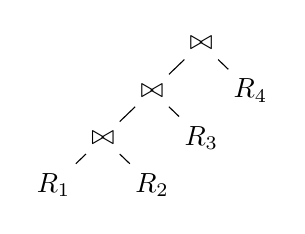
\begin{tikzpicture}[
			level distance=0.6cm,
			level 1/.style={sibling distance=1.25cm}
        ]
			\node { $\bowtie$ }
				child { node {$\bowtie$} edge from parent[-]
    				child { node {$\bowtie$} edge from parent[-]
                        child { node {$R_1$} edge from parent[-] }
                        child { node {$R_2$} edge from parent[-] }
                    }
                    child { node {$R_3$} edge from parent[-] }
                }
                child { node {$R_4$} edge from parent[-] };
		\end{tikzpicture}
        \caption{A width-2 query plan}
        \label{fig:non-hierarchical-plan}
    \end{subfigure}
    \caption{The hypergraph, a join tree, a width-1 query plan, and a width-2 query plan of the query $Q_{\ref{ex:hierarchical}}$}
    \label{fig:hierarchical}
\end{figure}
